\section{Load Balance}

For addressing a load balance issue, we first need to characterize the source of the imbalance. The asymmetry can come from an improper work distribution or different instructions per cycle.


To characterize the imbalance source, we need a way to determine how the application is distributing the work.

Equation \ref{eq:IB} shows the useful instruction balance (UIB) calculation, which essentially computes how the application is distributing the work. 

 \begin{equation}\label{eq:IB}
   UIB=\frac{avg_{i=1}^{|P|}I_{U_i}}{max_{i=1}^{|P|}I_{U_i}}
\end{equation}


With Paraver, we obtained the useful instructions of each run's process and computed the useful instruction balance. Figure \ref{lbchar} shows the comparison between the useful instruction balance and the load balance. We can see that the work distribution is the main issue affecting the application balance. 

\begin{figure}[h]
  \centering
  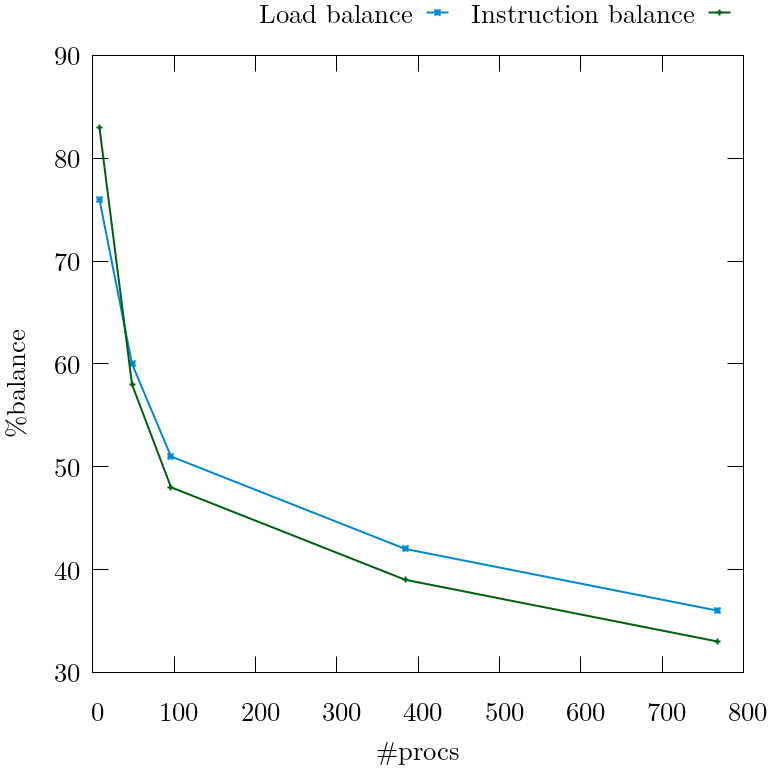
\includegraphics[width=0.5\textwidth]{loadbalance-comp}
  \caption[Load balance characterization.]{Load balance characterization. Own compilation.}
  \label{lbchar}
\end{figure}



